\chapter{Durchführung}
\label{cha:Durchführung}
In Abbildung \ref{fig:aufbau} ist der Versuchsaufbau dargestellt. Die Maße des Detektors selber sind der Abbildungs zu entnehmen. Die aufgedampfte Lithiumschicht ist 
$d_\mathrm{Li} = \qty{0.5}{\centi\metre}$ dick. Die Goldschicht ist $d_\mathrm{Au} = \qty{20}{\micro\metre}$ dick. Um den Detektor ist eine Aluminiumhülle aufgebaut, welche zum 
Schutz dient. Rechts in Abbildung \ref{fig:aufbau} sind die NIM-Standard Module zur Datenerfassung aufgebaut. Nach dem Amplifier werden die Daten durch einen Multi-Channel-Analyser
aufgenommen und abgespeichert.

\begin{figure}
    \centering
    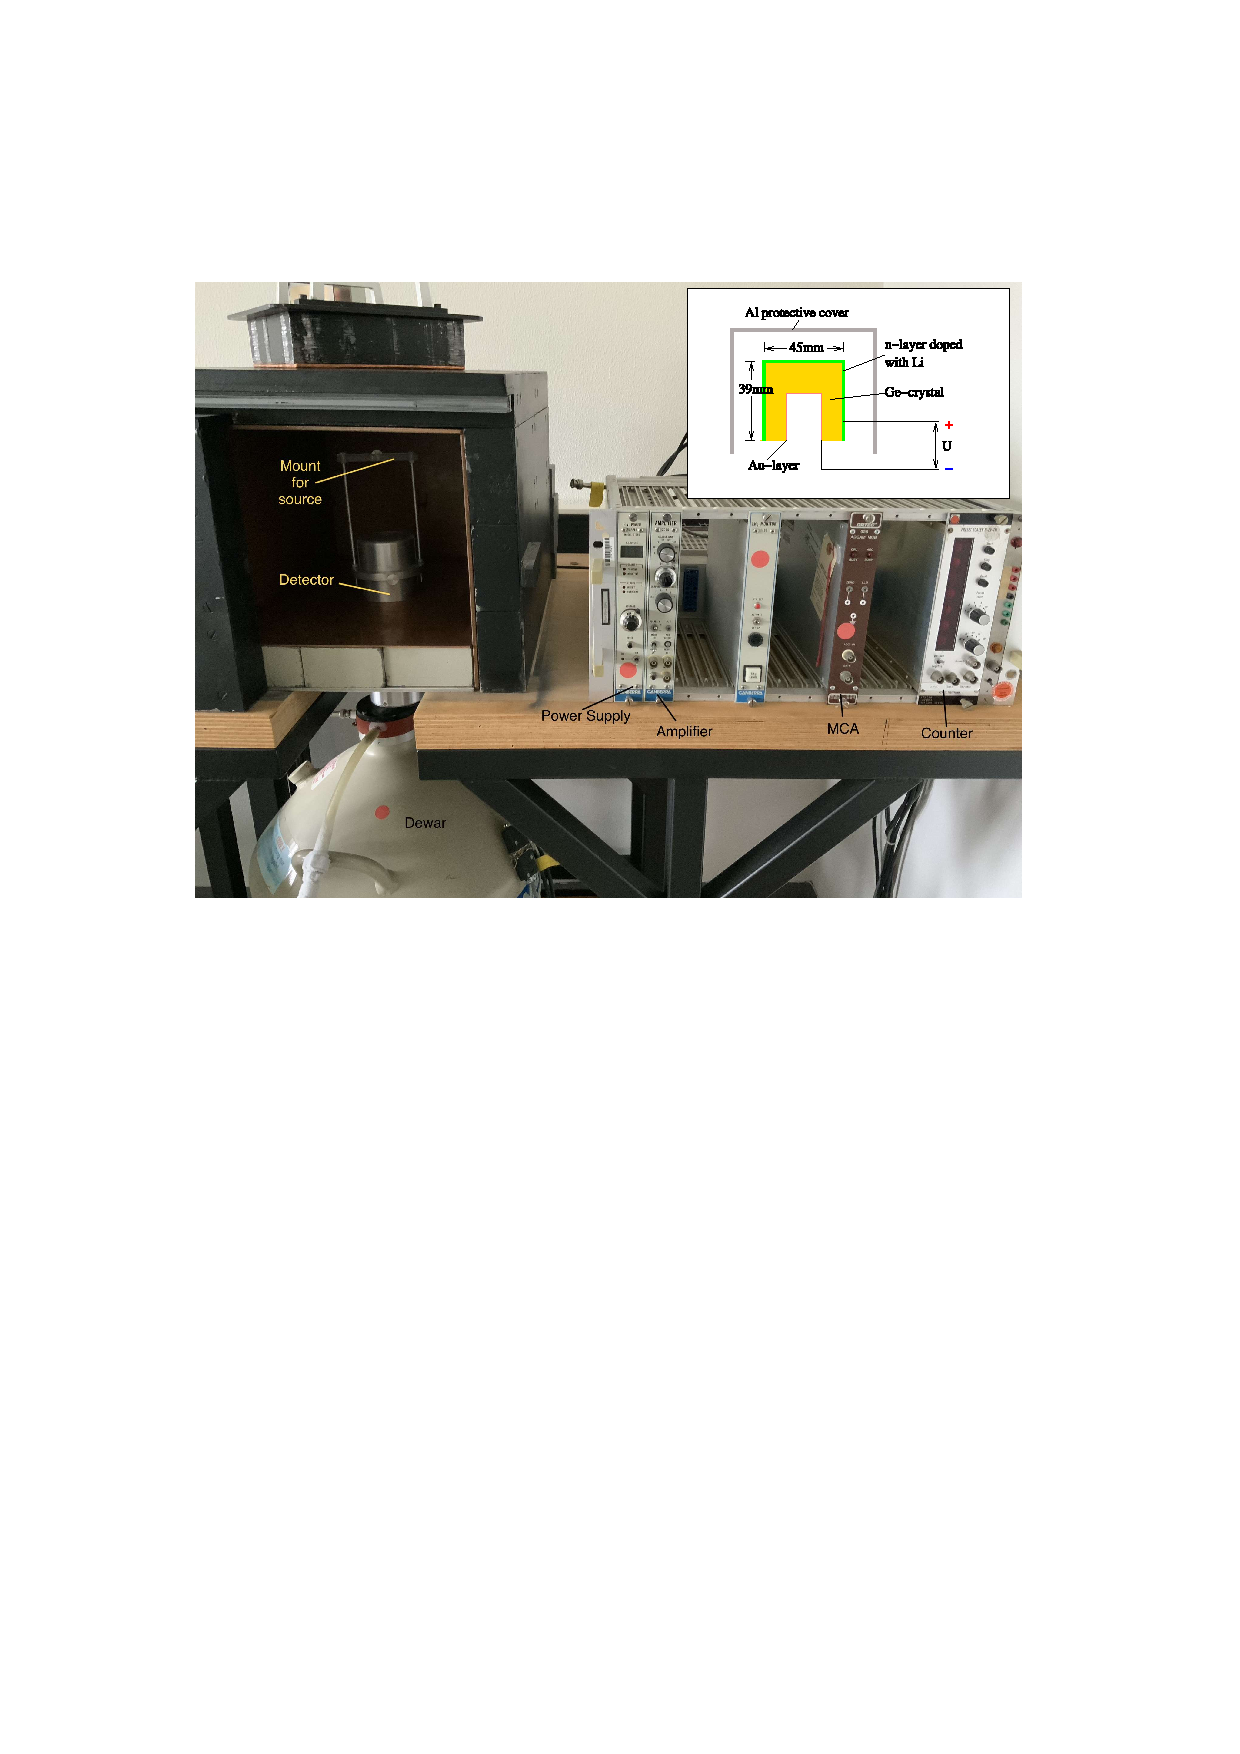
\includegraphics[width = .9\textwidth]{content/pics/aufbau.pdf}
    \caption{Bild des Versuchsaufbaus.}
    \label{fig:aufbau}
\end{figure}

Die Gammastrahler werden oberhalb des Detektors in einem Abstand von $d = \qty{7.01 +- 0.005}{\centi\metre}$ fixiert.

Zu Beginn des Versuches werden aller nötigen geometrischen Längen gemessen. Danach wird der Detektor in Betrieb genommen und eine Energiekalibration wird vorgenommen. Außerdem wird 
Energiedetektionswahrscheinlichkeit des Detektors gemessen, indem das Spektrum des bekannten $\ce{^{152}_{63}Eu}$-Strahlers verwendet wird. Nun ist der Detektor bereit für 
Messungen. 

Daraufhin wird das Spektrum einer $\ce{^{137}_{55}Cs}$ Probe aufgenommen. Je nach Aktivität der Probe wird eine Messdauer von einer dreiviertel Stunde angesetzt. 

Weiter wird das Spektrum einer völlig unbekannten Probe aufgenommen. Aus dem Spektrum soll die Probe bestimmt werden. 

Zuletzt wird das Spektrum eines unbekannten komplexen Strahlers aufgenommen. Komplex bedeutet, dass es sich nicht um eine reine Probe handelt. sondern um eine Probe aus mehreren 
Strahlern. Auch diese soll dadurch charakterisiert werden. 